\documentclass[conference]{IEEEtran}
%\IEEEoverridecommandlockouts
% The preceding line is only needed to identify funding in the first footnote. If that is unneeded, please comment it out.
\usepackage{cite}
\usepackage{amsmath,amssymb,amsfonts}
\usepackage{algorithmic}
\usepackage{graphicx}
\usepackage{textcomp}
\usepackage{xcolor}
\usepackage{tikz}
\usetikzlibrary{arrows.meta}
\usetikzlibrary{chains}
\usepackage{fontawesome5}

%% TODONOTES
\paperwidth=\dimexpr \paperwidth + 6cm\relax
\oddsidemargin=\dimexpr\oddsidemargin + 3cm\relax
\evensidemargin=\dimexpr\evensidemargin + 3cm\relax
\marginparwidth=\dimexpr \marginparwidth + 3cm\relax
\usepackage{todonotes}

\begin{document}

\title{Telling the Time: Modern-Day Complications}
%\thanks{Identify applicable funding agency here. If none, delete this.}

\author{\IEEEauthorblockN{Vincent Bode}
\IEEEauthorblockA{\textit{Department of Computer Science} \\
\textit{Technical University of Munich}\\
Munich, Germany \\
vincent.bode@tum.de}
\and
\IEEEauthorblockN{Arpan Gujarati}
\IEEEauthorblockA{\textit{Systopia Lab} \\
\textit{University of British Columbia}\\
Vancouver, Canada \\
arpanbg@cs.ubc.ca}
%\and
%\IEEEauthorblockN{3\textsuperscript{rd} Given Name Surname}
%\IEEEauthorblockA{\textit{dept. name of organization (of Aff.)} \\
%\textit{name of organization (of Aff.)}\\
%City, Country \\
%email address or ORCID}
}

\maketitle

\begin{abstract}
\end{abstract}

\begin{IEEEkeywords}
PTP, Time Synchronization, Fault Tolerance
\end{IEEEkeywords}


\section{Introduction}
\todo{Find places to insert the word ``real-time'' to solidify applicability to RTSS.}
%``Time is of the essence'', to many readers this might only be an idiom but the relevance of time throughout our daily lives, processes and systems is so ubiquitous that we frequently fail to appreciate its significance. While the phrase is said to have originated from the legal domain, time-criticality and the necessity of having a common notion of time permeates all sectors, from logistics and manufacturing in industry, to service-level objectives in service providers, emergency response in public healthcare systems, activities in people's day-to-day routines, and even to academia, as everybody perpetually works towards the next deadline. In computer systems and communications, time has been with us from the very beginnings, with its significance showing from the most basic synchronized digital circuits even to places where one might not expect, such as in the world's most pervasive digital cryptography deployment, the SSL/TLS PKI~\cite{ssl-client-warnings}.

Time is both ubiquitous and critical, no computer system today can run without it. With the availability of the internet, satellite communications and digital clocks, we take for granted that we can tell the time anywhere and anytime.
%
%Nowadays, with the availability of the internet, satellite communications and digital clocks, we often take for granted that we can tell the time anywhere and anytime. And for most human use cases, a rough estimate of the current time on the order of magnitude of seconds is perfectly sufficient.
%After all, sub-second granularity is irrelevant as people follow their daily schedules, and for project plans that span years or even decades a day or two more will not make a difference. \todo{colloquial/irrelevant}
However, in communications, real-time systems and circuitry, we operate on a scale where things are not so simple, with sub-nanosecond-level accuracies gaining significance in areas like networks and chip design~\cite{nanopu,sub-nanosecond-comms-design}.

Global Navigation Satellite Systems (GNNS), a classical application enabled by precision time-synchronization, relies on signal propagation delays to determine relative positioning~\cite{intro-to-gnss}.
High-quality location estimates hinge on accurate timing and -compensation mechanisms, so GNSS is frequently leveraged as a nanoscale clock source~\cite{gnss-location-and-time-advances,gnss-for-high-precision-timing}.
%Failure to compensate clock differences or even the presence of adversarial signals can quickly degrade the resulting location quality~\cite{gps-jamming}, but in general GNNS systems enjoy widespread popularity not only as a way of acquiring location estimates but also as a way of obtaining highly accurate estimates of time~\cite{gnss-location-and-time-advances,gnss-for-high-precision-timing}.
The precision incurs expense though, it requires dedicated hardware, strains limited power budgets, and inhibits e.g. indoor deployments.

Timing is also critical for fault-tolerant systems. Architectures such as double- or triple-modular lock-step redundancy~\cite{triple-modular-redundancy,triple-modular-redundancy-evaluation,triple-modular-lock-step-arm}, where algorithms are run independently on different machines to automatically detect and correct errors, rely on a common notion of time and deadlines to make progress even when a machine has failed. Such systems are found frequently in high-reliability and -availability applications such as aviation, where computer systems are relied on for controlling machinery with strict timing requirements.
%Failed safety-critical redundancy engineering has seen some infamous examples recently, with deadly Boeing 737-Max incidents prompting the introduction of new laws for flight control computer error resilience~\cite{boeing-requirements}\todo{better citation}.
\todo{@Arpan I removed the example, it's too much for the intro.}
Without a common notion of time, it would not be possible for resilient systems to judge internally missed deadlines correctly, thus preventing the system from providing proper error-detection and correction, voiding the fault-tolerance it was designed for.

However, time is not only critical in fault-tolerant systems, it pervades all distributed systems.
High-performance and datacenter computing are areas large amounts of resources are being spent on maximizing hardware utilization by reducing I/O or communications bottlenecks~\cite{hpc-understanding-bottlenecks, hpc-solving-io-bottleneck, hpc-diagnosing-io-bottlenecks}, and a common notion of time is a prerequisite enabling technology to effective profiling and optimization on distributed systems.
%The better the time source, the easier it becomes to perform efficient handovers by precise scheduling, thus improving overall performance and resource consumption.
Google and Facebook\todo{cite} have come up with time synchronization implementations based on the notion of windows of uncertainty that can be used to ensure transaction ordering across a distributed system without an application having to explicitly synchronize, a property useful not only to databases but also to real-time control, fault detection/mitigation and parallel data structures.
Time synchronization techniques also transfer to edge computing, where scheduling computation and communication to efficiently manage load can conserve power and connectivity resources, allowing applications to achieve more with less hardware.
Even large scale deployments like the internet cannot function without timing, as SSL/TLS cryptographic certificate validation, renewal of leases (DHCP) and caches (DNS, HTTP), and various other state machines built into systems and protocols (TCP, firewalls, etc.) all rely on clocks to function.

Clearly, clock synchronization is essential in almost all aspects of computing, and there is a broad range of accuracies that we need to keep time in. But to what degree we can truly rely on modern computer timekeeping in distributed embedded systems when failures affect correctness?
We need to evaluate what our systems are capable of and what sort of reliability guarantees they can provide for our algorithms to work with.
Especially in industrial and embedded computing/IoT, deployments are often characterized by dependability/redundancy requirements and a general necessity to conserve all types of resources to reduce costs, as well as their relative isolation regarding connectivity.
This sets it apart from more traditional computer timekeeping scenarios, where an external source of truth can be relied upon, here internal consistency is the primary motivation.
%Good timekeeping allows a reduction in the amount of comparatively resource-intensive manual synchronization required, which directly leads to cost savings, however a high level of trust in the clock is needed to ensure ordering correctness. Across distributed embedded systems, we can use local network time synchronization to achieve this, however the question of accuracy and dependability under adverse conditions is open.
Before we can trust a synchronization algorithm, we need to understand how it performs and what causes it to break, which is what we will be investigating throughout the rest of this paper.
%\todo{Need a part here on what we are actually doing.}
%\todo{Dependable embedded systems.}


We evaluate the performance and resilience of four implementations of prevalent time synchronization protocols for packet-switched Ethernet networks, including the Precision Time Protocol (PTP) and the Network Time Protocol (NTP), across four hardware testbeds, showing strengths and weaknesses in a variety of configurations. We offer the following contributions:

\begin{itemize}
    \item Development of a tool, PTP-Perf, for fair and comparable cross-vendor evaluation of multiple time synchronization protocols and implementations,
    \item Establishment of a baseline of observed time-synchronization performance on several hardware testbeds across four vendors,
    \item Evaluation of synchronization resilience against adverse conditions/faults and possibilities of mitigating risk of synchronization failure,
    \item Assessment of deployability/resource consumption on embedded platforms,
    \item Provide lessons-learned and best practices for configuring time-synchronization deployments for high reliability and availability.
\end{itemize}

To the best of our knowledge, with PTP-Perf we provide the first data collection and analysis tooling available open-source\todo{anonymize} that supports the empirical evaluation of multiple Ethernet-based time synchronization protocols and implementations across several embedded hardware testbeds with an explicit focus on dependability and fault-tolerance.
%We also make the data collection and analysis tooling available open-source\todo{anonymize} to enable future studies to generate comparable results.
%
The rest of this paper is structured into the following sections: Section~\ref{sec:background} covers time synchronization and PTP background, as well as related work, while Section~\ref{sec:failure_scenarios} looks at potential failure scenarios. Results are presented in Sections~\ref{sec:baseline} Baseline, \ref{sec:resource_contention} Resource Contention, \ref{sec:fault_tolerance} Fault Tolerance and \ref{sec:resource_consumption} Resource Consumption. Finally, we present some lessons learned and best practices in Section~\ref{sec:learnings_conclusion}.

%\section{Applications that Require Time}
%\label{sec:motivation}



\section{Time Synchronization \& PTP}

Over the years, many different algorithms and solutions to time synchronization across computer networks have been explored [cite]. In today's most widely deployed network stack for general purpose computing, IP, two protocols have established themselves as standard for time synchronization: the Network Time Protocol (NTP) for Wide Area Networks (WANs) and the Precision Time Protocol (PTP) for Local Area Networks (LANs) that require a greater degree of time synchronization precision. Both protocols are standardized and each have multiple implementations available at the time of writing. Alternatives also include SPTP, a simplified version of PTP developed by Meta that claims to offer comparable performance to PTP while reducing resource consumption [cite].

Because we are interested in evaluating time synchronization for dependable systems, we will focus on PTP as it is designed to be deployed in controlled environments such as a fault-tolerant control network. PTP has wide-spread adoption and also serves as a foundation for technologies such as IEEE Time Sensitive Networking (TSN).


\subsection{PTP -- Background and Architecture}

PTP operates across a network and has two types of endpoints: master nodes and slave nodes. A PTP master provides synchronization signals to the slaves (Figure \ref{fig:ptp-architecture}), which each use the synchronization signal in combination with a path delay estimate to determine an estimate of the local clock offset to the master clock, which is subsequently used to discipline the local clock to keep it synchronized with the master's clock. While the actual protocol is slightly more complex and includes additional messages for synchronization leases and state management, the two core message types are sufficient in principle to synchronize the system clocks. Note that it is assumed that the PTP master already has a high-quality clock source for the current time -- preferably an external source like an atomic clock or a GPS signal, but the master clock can also be obtained from e.g. a different PTP domain.

\begin{figure}
    \begin{tikzpicture}[client/.style={draw}, message/.style={midway, above, sloped, inner sep=0mm}, on grid]
        \node[client] (master) {PTP Master};
        \node[client, above=of master] (clock) {\faClock[regular]};
        \draw[thick, dotted] (master) -- (clock);

        \node[client, right=1.75cm of master] (switch) {\faNetworkWired};
        \draw[-Stealth] (master) -- (switch);

        \foreach \i in {1,...,3}{
            \node[client] (slave-\i) at (3.5, \i - 2) {PTP Slave};
            \draw[-Stealth] (switch) -- (slave-\i.west);
        }

        \begin{scope}[xshift=5.5cm, yshift=2cm]
            \node (master) at (0,0) {Master};
            \node (slave) at (2,0) {Slave};

            \draw[-] (master) -- ++(0, -3.75);
            \draw[-] (slave) -- ++(0, -3.75);

            \foreach \i in {0.5, 1, 1.5}{
                \draw[-Stealth] (0, -\i) -- ++(2, -0.5) node[message] {Sync};
            }

            \draw[-Stealth] (2, -2.5) -- ++(-2, -0.5) node[message] {Delay Req.} -- ++(2, -0.5) node[message, below, inner sep=0.5mm] {Delay Resp.};
        \end{scope}
    \end{tikzpicture}
    \caption{
        A PTP master provides a synchronization signal to a number of slaves so that they can keep their local clock synchronized to the master's clock (left). The clock synchronization relies on two types of signals (right): a periodic synchronization signal to distribute the current master time and the delay request/response to estimate the propagation delay.
    }
    \label{fig:ptp-architecture}
\end{figure}

\subsection{PTP Profiles}
PTP is built to be configurable, settings include anything from the underlying transport (unicast/multicast), the delay mechanism to use (end-to-end or peer-to-peer), message frequencies and leases, as well as rules to discipline the clock. To reduce the complexity of configuring PTP, several so-called profiles are available that provide default settings for the specific use-case. \todo{Provide example profiles} To conduct our evaluation, we use each vendor's default profile, as this profile is the one that runs on general purpose deployments without special configuration, and is therefore the one that most users will come in contact with.

\subsection{Synchronization Performance}
It is generally understood that network clock synchronization accuracy is a function of the signal propagation delay and its variance [cite]. A naive approach to clock synchronization that just sends a timestamp from the master to the slave would always be off by the propagation delay, but PTP uses path delay estimation to try and compensate for the propagation delay thus increasing the accuracy. In an ideal world where there is no packet delay variation, the propagation delay could be mitigated entirely, but in reality we have multiple software and hardware components, like the kernel, network stack and network hardware, that each introduce latency variability, which in turn worsens the performance of the delay compensation. Effects such as asymmetric latencies caused by uneven loads that cannot easily be compensated for further reduce the synchronization accuracy. Thus, limiting the packet delay variation becomes a primary concern when tuning for precision and dependability.

\subsection{Hardware Acceleration}

\begin{figure}
    \newcommand{\timestampClock}[1][100]{\textcolor{black!#1}{\faClock[regular]}}

    \begin{tikzpicture}[
        start chain=components going below,
        start chain=components2 going below,
        component block/.style={draw, minimum height=0.75cm},
        node distance=0cm,
    ]

            \begin{scope}[name prefix=stack1-, component/.style={component block, text width=3.5cm}]
                \node[on chain=components, component] at (0, 0) (PTP) {PTP Client \hfill \rotatebox{45}{\faStamp{}} \timestampClock{} \faEnvelope[regular]};
                \node[on chain=components, component] (Kernel) {Kernel \hfill \timestampClock[60] \faEnvelope[regular]};
                \node[on chain=components, component] (IP-Stack) {IP Stack \hfill \timestampClock[40] \faEnvelope[regular]};
                \node[on chain=components, component] (Hardware Queue) {Hardware Queue \hfill \timestampClock[30] \faEnvelope[regular]};
                \node[on chain=components, component] (NIC) {NIC \faEthernet \hfill \timestampClock[20] \faEnvelope[regular]};

                \node[above=of PTP] (title) {Software PTP};
            \end{scope}

            \begin{scope}[name prefix=stack2-, component/.style={component block, text width=3.5cm}]
                \node[on chain=components2, component] at (5.5, 0) (PTP) {\faEnvelope[regular] \hfill PTP Client};
                \node[on chain=components2, component] (Kernel) {\faEnvelope[regular] \hfill Kernel};
                \node[on chain=components2, component] (IP-Stack) {\faEnvelope[regular] \hfill IP Stack };
                \node[on chain=components2, component] (Hardware Queue) {\faEnvelope[regular] \hfill Hardware Queue};
                \node[on chain=components2, component] (NIC) {\faEnvelope[regular] \faClock[regular] \rotatebox{-45}{\faStamp{}}  \hfill \faEthernet{} NIC};

                \node[above=of PTP] (title) {Hardware PTP};
            \end{scope}

            \draw[Stealth-Stealth, very thick] (stack1-NIC) -- (stack2-NIC) node[midway, draw, fill=white] (network) {\faNetworkWired};

            \node[draw, dashed, below=0.25cm of network] (network-annotation) {\faClock[regular] $\rightarrow$ \faHistory{}\,\textsuperscript{\textbf{*}}};
            \draw[dotted] (network.south west) -- (network-annotation.north west);
            \draw[dotted] (network.south east) -- (network-annotation.north east);

    \end{tikzpicture}
    \caption{
        Timestamping for PTP messages when using software timestamping (left) and hardware timestamping (right). For software timestamping, the timestamp is generated inside the PTP client and traverses many layers in both egress and ingress, causing additional path delay and delay variation. With hardware timestamping, a timestamp is only added to the message just before it is written to wire by the NIC, thus ensuring a more up-to-date timestamp is sent to the network.\\
        \textsuperscript{\textbf{*}}Network hardware (switches, routers, etc.) also introduces queuing delays. Special PTP-aware hardware can compensate for its own delays to further improve timestamping quality.
    }
    \label{fig:ptp-sw-hw}
\end{figure}

Since delay variation is a primary concern, hardware techniques have been developed to reduce the variability. While PTP can run entirely in software, the path that packets need to traverse between two PTP clients not only includes several hardware components but also some software layers (Figure~\ref{fig:ptp-sw-hw} left). Each component along the path introduces latency and packet delay variation, deteriorating the signal quality. With the appropriate hardware support, message timestamps can instead be generated directly by the NIC driver/hardware (Figure~\ref{fig:ptp-sw-hw} right), which ensures that the timestamp is not affected by the layers above it. This increases the clock synchronization's resilience against interference from adverse conditions, such as high network-, CPU- or kernel load.

\section{Methodology}

\subsection{Testbed -- Hardware and Software}

\subsection{PTP Lifecycle}

\begin{figure*}
    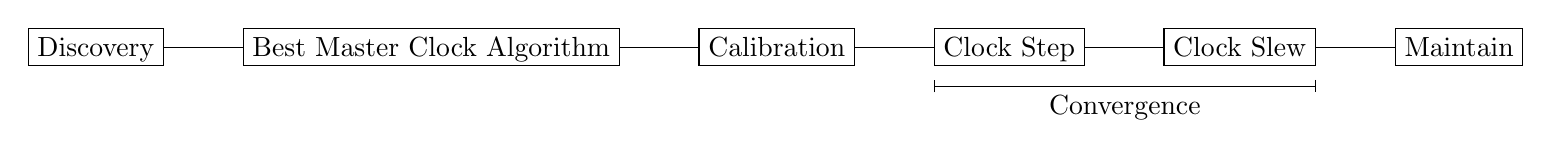
\begin{tikzpicture}[
        start chain=stages going right,
        stage/.style={
            draw, on chain=stages,
            every on chain/.style={join}, every join/.style={-Stealth}
        },
        text depth=0cm,
        ]
        \node[stage] {Discovery};
        \node[stage] {Best Master Clock Algorithm};
        \node[stage] (calibrate) {Calibration};
        \node[stage] (step) {Clock Step};
        \node[stage] (slew) {Clock Slew};
        \node[stage] {Maintain};

        \draw[Bar-Bar] ([yshift=-0.25cm]step.south west) -- ([yshift=-0.25cm]slew.south east) node[midway, below] {Convergence};
    \end{tikzpicture}
    \caption{Different stages in the PTP lifecycle that a PTP client traverses while synchronizing its clock. }
\end{figure*}

PTP clients traverse multiple stages in a lifecycle to synchronize their clock.

\end{document}